\part{Up layer}
\label{up_layer}

Vrchní vrstva přenášená data (ta která si vyměnuje se spodní vrstvou) zpracovává a to vždy po celých kusech. V kontextu vrchní vrstvy (vrstvy CRPP) se monolitické bloky dat označují jako ``message". Každá message je ucelený soubor dat (posloupnost bytů), který je možné jednotlivě zpracovat. Datová struktura a způsob zpracování message je popsáno v části \ref{up_layer.collab_message}, použité datový typy v části \ref{connection.data_types}.

\chapter{Collab message}
\label{up_layer.collab_message}

CRPP message je posloupnost bytů. Každá message má význam příkazu (požadavku na vykonání nějaké funkce) a může obsahovat parametry.

\section{Message}

Message se skládá ze dvou částí a to z jejího příkazu a nepovinných parametrů. Příkaz reprezentují 4 ASCII znaky (4 byty). Parametry nemusí message vůbec obsahovat a může jich být neomezené množství. Jejich struktura je popsána v části \ref{up_layer.collab_message.parameter}.

Obsah message je také ilustrován obrázkem \ref{up_layer.pictures.message_structure}.

\begin{figure}[h]
  \centering
  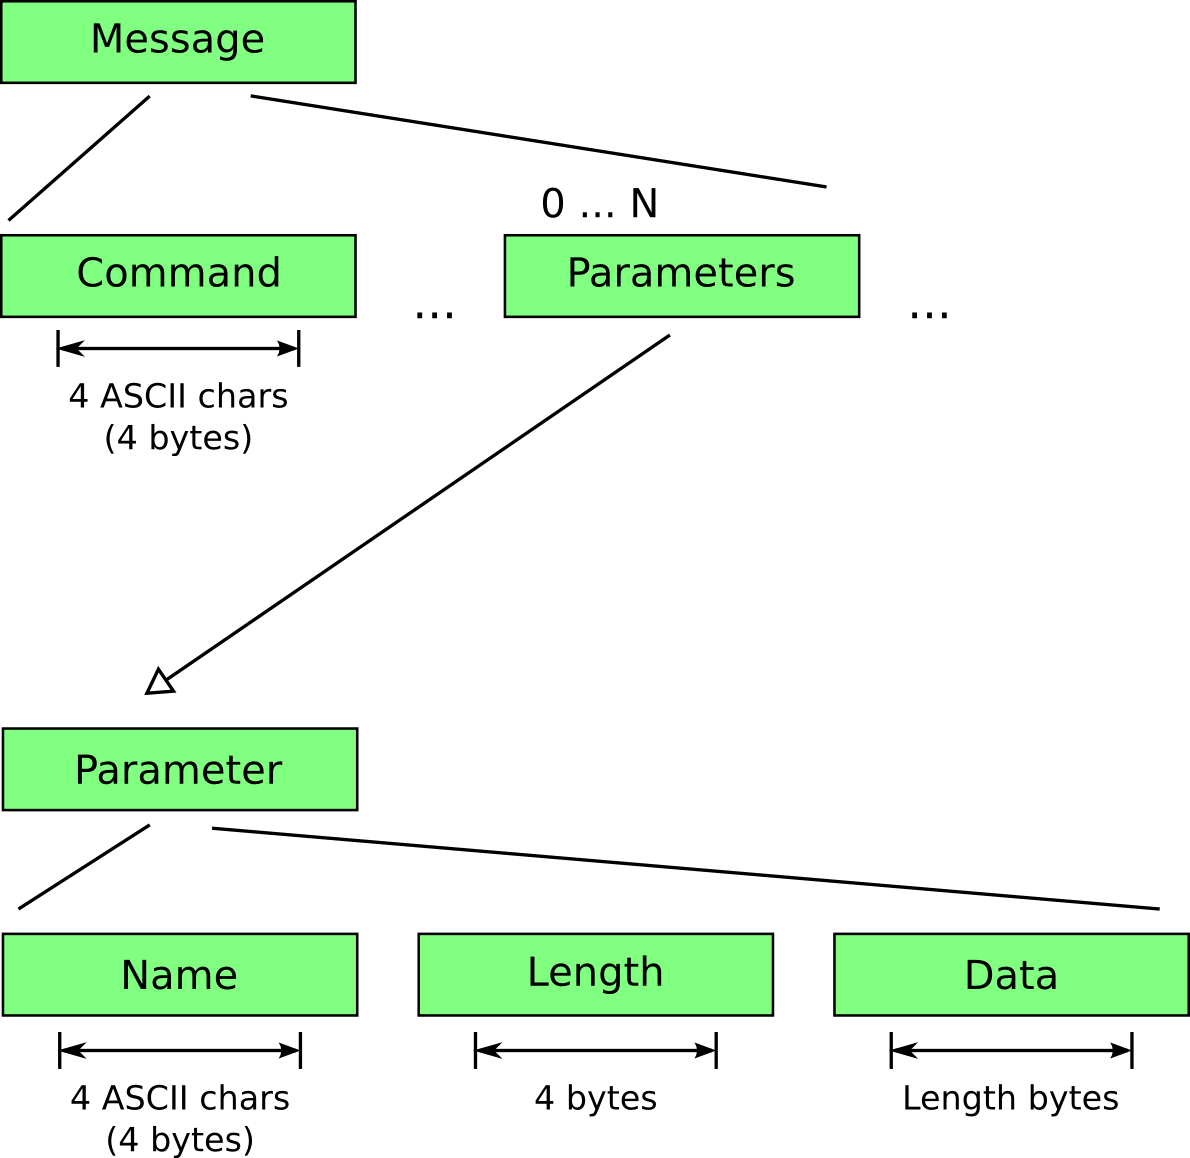
\includegraphics[width=0.80\textwidth]{diagrams/message_structure_diagram.png}
  \caption{Message structure diagram}
  \label{up_layer.pictures.message_structure}
\end{figure}

\section{Parameter}
\label{up_layer.collab_message.parameter}

Každý paremetr je reprezentován jako blok dat. Obsahuje tyto části:

\begin{enumerate}
	\item paremeter name (4\,{}B)
	\item data length (4\,{}B)
	\item parameter data (data length\,{}B)
\end{enumerate}

První část (paremeter name) jsou 4 ASCII znaky (4 byty), které jednoznačně identifikují parametr. Následující 4 byty udávají jako neznaménkové celé číslo délku dat ($n$). Dalších $n$ bytů jsou data parametru. Data jsou interpretována různě podle toho v jakém příkazu je parametr obsažen a v jakém parametru jsou obsaženy data. Základní používané datové typy jsou posány v části \ref{connection.data_types}.

V části \ref{commands} jsou popsány jednotlivé příkazy, jejich parametry, význam a způsob zpracování.